\documentclass[
  convert={
    size=1080x800,
    outext=.png
  },
]{standalone}
\usepackage{tikz} 
\usetikzlibrary{decorations.markings} 

\usepackage[icelandic]{babel}
\usepackage[utf8x]{inputenc}
\usepackage[T1]{fontenc}
\usepackage{xcolor}

\definecolor{myyellow}{RGB}{254,241,24}
\definecolor{myorange}{RGB}{234,125,1}

\begin{document}

\nopagecolor

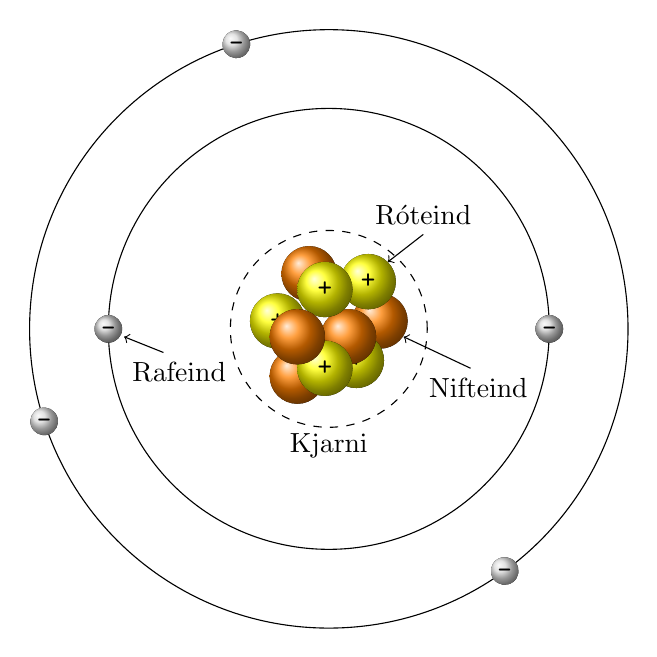
\begin{tikzpicture}
\def\proton(#1,#2){%
    \fill[shading=ball,ball color=yellow] (#1,#2) circle (10pt);
    \node at (#1,#2) {\texttt{+}};
}
\def\neutron(#1,#2){%
    \fill[shading=ball,ball color=orange] (#1,#2) circle (10pt);
}
\def\electron{%
    \fill[shading=ball,ball color=gray!30] (0,0) circle (5pt);
    \node at (0,0) {\texttt{-}};
}
\neutron(0.65,0.1)
\proton(0.35,-0.4)
\neutron(-0.4,-0.6)
\proton(0.5,0.6)
\proton(-0.65,0.1)
\neutron(-0.25,0.7)
\neutron(0.25,-0.1)
\proton(-0.05,0.5)
\proton(-0.05,-0.5)
\neutron(-0.4,-0.1)
\draw[
  postaction=decorate,
  decoration={markings, 
  mark=at position 0.5 with {\electron},
  mark=at position 1 with {\electron}
}] 
  (0,0) circle (2.8cm);
\draw[
  postaction=decorate,
  decoration={markings, 
  mark=at position 0.3 with {\electron},
  mark=at position 0.55 with {\electron},
  mark=at position 0.85 with {\electron},
}] 
  (0,0) circle (3.8cm);
  
\draw [dashed] (0,0) circle (1.25cm) node[below,yshift=-1.2cm] {Kjarni};

\draw [<-] (0.75,0.85) -- (1.2,1.2) node[above] {Róteind};
\draw [<-] (0.95,-0.1) -- (1.8,-0.5) node[below,xshift=0.1cm] {Nifteind};
\draw [<-] (-2.6,-0.1) -- (-2.1,-0.3) node[below,xshift=0.2cm] {Rafeind};

\end{tikzpicture}

\end{document} 